\section{应用程序实现}\label{sec:ApplicationsImplementation}

在本节(\cref{sec:ApplicationsImplementation})中,笔者将详细探讨在MinmusOS上实现的一个示例应用程序——汉诺塔解决方案。这个示例应用程序不仅展示了基于Rust的系统级编程实践,也具体演示了如何在裸机或类似环境下运行复杂的应用程序。

\subsection{应用程序构建脚本}

apps/hanoi/build.rs构建脚本(\cref{lst:AppsHanoiBuildRust})的主要功能是为Rust编译器配置特定的链接器脚本,以便正确地编译和链接汉诺塔应用程序。以下是详细介绍:

\begin{enumerate}
    \item \textbf{环境变量读取}:脚本使用 \texttt{env!("CARGO\_MANIFEST\_DIR")} 来获取当前包的清单(Manifest)目录。这个环境变量是由Cargo设置的,指向你的项目的根目录,即包含 Cargo.toml 的目录。
    \item \textbf{路径拼接}:通过 \texttt{std::path::Path::new} 将获取到的目录转换为一个路径对象,然后使用 join 方法拼接上 linker.ld。这样操作是为了构造出链接器脚本的完整路径。
    \item \textbf{链接器参数设置}:脚本使用 \texttt{println!} 输出一个特殊的编译器指令,这条指令会被Cargo捕捉并用于配置编译过程。具体来说,\texttt{cargo:rustc-link-arg-bins} 告诉Rust编译器在编译二进制文件时应该使用指定的链接器脚本。
\end{enumerate}

\begin{listing}[htbp]
    \begin{minted}{rust}
fn main() {
    let local_path = std::path::Path::new(env!("CARGO_MANIFEST_DIR"));
    println!("cargo:rustc-link-arg-bins=--script={}", local_path.join("linker.ld").display());
}
    \end{minted}
    \caption{apps/hanoi/build.rs}\label{lst:AppsHanoiBuildRust}
\end{listing}

在操作系统内核中实现应用程序时,构建脚本起到的关键作用是确保应用程序能够与内核适当地链接,以便在内核的上下文中正确执行。使用自定义的链接器脚本,可以精确控制程序的内存布局、符号解析等关键方面,这些都是在裸机或自定义操作系统上运行代码的必要条件。通过这种方式,可以确保应用程序的代码和数据被放置在内核预期的特定位置,使得程序能够在没有标准操作系统支持的环境中运行。

\subsection{应用程序链接器脚本}

应用程序的链接器脚本(\cref{lst:HanoiLinkerScript})是定义程序在内存中的布局的关键文件。该脚本指定了程序的各个部分应该放在内存的哪个位置,以及如何组织这些部分。

\begin{listing}[htbp]
    \begin{minted}{text}
/* 配置程序入口点 */
ENTRY(_start)

/* 配置段的顺序和位置 */
SECTIONS {
    /* 定义起始内存地址 */
    . = 0x02000000;

    /* 定义应用程序开始标记 */
    .start_marker :
    {
        LONG(0xB16B00B5)
    }

    /* 定义应用程序起始点 */
    _app_start = .;

    /* 定义启动段,包含启动代码的实际入口点 */
    .start : {
        *(.start)
    }

    /* 定义代码段,包含程序的机器代码 */
    .text : {
        *(.text .text.*)
    }

    /* 定义 BSS 段,包含程序中未初始化的数据 */
    .bss : {
        *(.bss .bss.*)
    }

    /* 定义只读数据段,包含常量等不应被程序修改的数据 */
    .rodata : {
        *(.rodata .rodata.*)
    }

    /* 定义数据段,包含已初始化的全局变量和静态变量 */
    .data : {
        *(.data .data.*)
    }

    /* 配置异常处理信息,用于支持运行时错误处理 */
    .eh_frame : {
        *(.eh_frame .eh_frame.*)
    }
    .eh_frame_hdr : {
        *(.eh_frame_hdr .eh_frame_hdr.*)
    }

    /* 在内存中设置一个结束标记,用于标识引导加载器的结束 */
    .end_marker :
    {
        SHORT(0xDEAD)
    }
}
    \end{minted}
    \caption{apps/hanoi/linker.ld}\label{lst:HanoiLinkerScript}
\end{listing}

\subsection{应用程序入口}

\cref{lst:ApplicationEntry}是应用程序与操作系统交互的起点,尤其是在裸机环境或自定义操作系统如MinmusOS中。这里的实现详细说明了如何初始化程序、处理异常,并确保程序可以在没有标准库支持的环境下运行。下面是各部分的具体介绍:

\begin{listing}[htbp]
    \begin{minted}{rust}
#![no_std]
#![no_main]

use core::panic::PanicInfo;

fn main() {
    ...
}

#[no_mangle]
#[link_section = ".start"]
pub extern "C" fn _start() {
    main();
    loop {}
}

#[panic_handler]
fn panic(_info: &PanicInfo) -> ! {
    loop {}
}
    \end{minted}
    \caption{apps/hanoi/src/main.rs}\label{lst:ApplicationEntry}
\end{listing}

\begin{enumerate}
    \item \textbf{属性指令}
          \begin{enumerate}
              \item \texttt{\#![no\_std]}:这条属性禁用Rust标准库。因为在裸机或内核模块中,标准库的某些部分(如堆内存分配、线程等)可能不可用。
              \item \texttt{\#![no\_main]}:通常Rust程序从标准的main函数开始执行。这个属性指示编译器程序将不从传统的main函数入口开始,这是因为在操作系统或裸机环境中,入口点通常是自定义的。
          \end{enumerate}
    \item \textbf{入口函数\_start}
          \begin{enumerate}
              \item \texttt{\#[no\_mangle]}:此属性用于防止编译器更改函数名称(即避免名称改编),确保链接时可以正确识别该函数。
              \item \texttt{\#[link\_section = ".start"]}:将此函数放置在特定的内存段,这里是.start段,正如链接器脚本中指定的。
              \item \texttt{pub extern "C"}:表示这个函数应遵循C语言的函数调用约定,这对于与其他语言或运行时环境交互是必要的。
              \item \texttt{main()}:函数体内调用\texttt{main()},之后进入无限循环,这样做是为了防止程序执行完毕后继续向下执行到未定义的内存区域。
          \end{enumerate}
    \item \textbf{Panic处理}
          \begin{enumerate}
              \item \texttt{\#[panic\_handler]}:这个属性定义了一个函数,用于处理程序运行中遇到的panic情况(即程序中的不可恢复错误)。
              \item \texttt{panic}:这个函数接收一个关于panic的信息对象,返回类型为\texttt{!},表示这个函数不会返回(即终止函数)。函数体中的无限循环确保在panic发生后,程序不会无序退出或执行未定义操作。
          \end{enumerate}
\end{enumerate}

此部分代码是整个程序能够在特定硬件或自定义操作系统上运行的基础。它确保了程序在启动时能够按照预定的方式初始化,同时在运行过程中遇到严重错误时有定义良好的行为。在不使用标准库的情况下,开发者需要手动处理所有的初始化和异常情况。

\subsection{应用程序实现}

这个汉诺塔解决方案应用程序是为MinmusOS操作系统内核编写的,完全使用Rust语言实现,不依赖于标准库,这意味着它能在裸机或极为简化的环境中运行。在程序的主函数中,首先初始化一个HanoiTowers结构体(\cref{lst:HanoiTowersDataStructure}),这个结构体包含三个数组,分别代表三根柱子,以及记录顶部位置和移动次数的变量。程序开始时,将从1到STACK\_SIZE的数字依次放入数组a,代表柱子A上从小到大的排列的圆盘。

\begin{listing}[htbp]
    \begin{minted}{rust}
struct HanoiTowers {
    a: [i32; STACK_SIZE],
    b: [i32; STACK_SIZE],
    c: [i32; STACK_SIZE],
    a_top: usize,
    b_top: usize,
    c_top: usize,
    count: usize,
}
    \end{minted}
    \caption{\texttt{HanoiTowers}数据结构}\label{lst:HanoiTowersDataStructure}
\end{listing}

\begin{listing}[htbp]
    \begin{minted}{rust}
fn main() {
    let mut towers = HanoiTowers {
        a: [0; STACK_SIZE],
        b: [0; STACK_SIZE],
        c: [0; STACK_SIZE],
        a_top: 0,
        b_top: STACK_SIZE,
        c_top: STACK_SIZE,
        count: 0,
    };
    for i in 0..STACK_SIZE {
        towers.a[i] = (i + 1) as i32;
    }
    println!("Hanoi Tower with {} disks:", STACK_SIZE);
    print!("#{:>4}     ", towers.count);
    print_stacks(&towers);
    move_disks(STACK_SIZE as i32, 'A', 'C', 'B', &mut towers);
}
    \end{minted}
    \caption{主函数}\label{lst:HanoiMainFunction}
\end{listing}

\begin{listing}[htbp]
    \begin{minted}{rust}
fn move_disks(n: i32, from: char, to: char, aux: char, towers: &mut HanoiTowers) {
    if n == 1 {
        move_one_disk(from, to, towers);
    } else {
        move_disks(n - 1, from, aux, to, towers);
        move_one_disk(from, to, towers);
        move_disks(n - 1, aux, to, from, towers);
    }
}

fn move_one_disk(from: char, to: char, towers: &mut HanoiTowers) {
    towers.count += 1;
    print!("#{:>4} {}->{}", towers.count, from, to);
    transfer_disk(from, to, towers);
    print_stacks(towers);
}

fn transfer_disk(from: char, to: char, towers: &mut HanoiTowers) {
    let (from_stack, to_stack, from_top, to_top) = match (from, to) {
        ('A', 'B') => (&mut towers.a, &mut towers.b, &mut towers.a_top, &mut towers.b_top),
        ('A', 'C') => (&mut towers.a, &mut towers.c, &mut towers.a_top, &mut towers.c_top),
        ('B', 'A') => (&mut towers.b, &mut towers.a, &mut towers.b_top, &mut towers.a_top),
        ('B', 'C') => (&mut towers.b, &mut towers.c, &mut towers.b_top, &mut towers.c_top),
        ('C', 'A') => (&mut towers.c, &mut towers.a, &mut towers.c_top, &mut towers.a_top),
        ('C', 'B') => (&mut towers.c, &mut towers.b, &mut towers.c_top, &mut towers.b_top),
        _ => return,
    };
    if *from_top < STACK_SIZE {
        let disk: i32 = from_stack[*from_top];
        from_stack[*from_top] = 0;
        *from_top += 1;
        if *to_top > 0 {
            *to_top -= 1;
            to_stack[*to_top] = disk;
        }
    }
}

fn print_stacks(towers: &HanoiTowers) {
    print!(" A ");
    for a in (0..STACK_SIZE).rev() {
        if a >= towers.a_top {
            print!("{:>2}", towers.a[a]);
        } else {
            print!("  ");
        }
    }
    print!(" B ");
    ...
    print!(" C ");
    ...
    println!();
}
    \end{minted}
    \caption{工具函数}\label{lst:HanoiUtils}
\end{listing}

\cref{lst:HanoiUtils}实现了汉诺塔解决方案应用程序的工具函数。程序调用move\_disks函数,这是一个递归函数,负责按照汉诺塔的规则移动圆盘,即每次只移动一个圆盘,并且任何时候较大的圆盘不能位于较小的圆盘之上。每次移动圆盘都会调用move\_one\_disk函数,这个函数更新圆盘的位置,记录移动次数,并调用print\_stacks函数打印当前柱子的状态。transfer\_disk函数则是处理实际的圆盘从一个数组到另一个数组的转移,确保不违反汉诺塔的移动规则。

程序的入口点是\_start函数,这是为了符合操作系统的启动要求,该函数将直接调用main函数(\cref{lst:HanoiMainFunction}),并在执行完毕后进入无限循环,防止程序退出到未定义的代码。异常处理由panic\_handler实现,当程序遇到不可恢复的错误时,它将进入另一个无限循环,确保系统不会无序地崩溃。整体而言,这个程序不仅是对经典汉诺塔问题的一个解决方案实现,也展示了在自定义操作系统中如何处理底层的程序逻辑和异常情况。

\cref{fig:ApplicationHanoiPresentation}展示了汉诺塔解决方案应用程序的运行。

\begin{figure}[htbp]
    \centering
    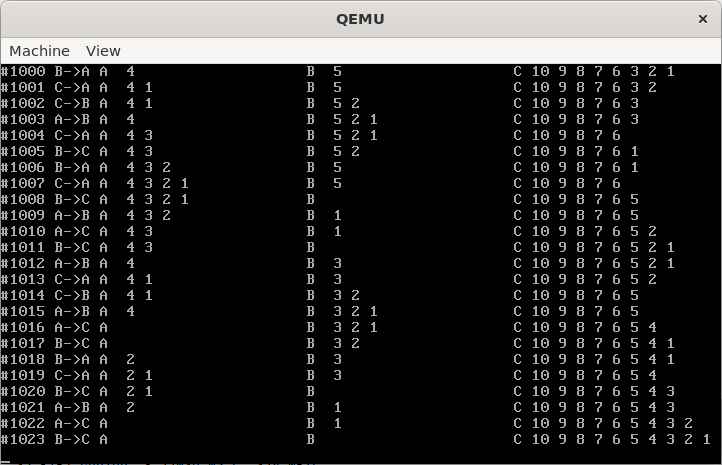
\includegraphics[width=0.8\textwidth]{figures/ApplicationHanoiPresentation.png}
    \caption{应用程序汉诺塔解决方案演示}
    \label{fig:ApplicationHanoiPresentation}
\end{figure}